\documentclass[11pt]{beamer}
\usetheme{Warsaw}
\usepackage[utf8]{inputenc}
\usepackage{amsmath}
\usepackage{amsfonts}
\usepackage{amssymb}
\usepackage{ctex}

\author{Jauntyliu @ SCGY-Tech}
\title{Lessons on Linux, Server and Git}
%\setbeamercovered{transparent} 
%\setbeamertemplate{navigation symbols}{} 
%\logo{} 
%\institute{} 
%\date{} 
%\subject{} 

\begin{document}

\begin{frame}
\titlepage
\end{frame}

%\begin{frame}
%\tableofcontents
%\end{frame}

\begin{frame}
\frametitle{What is PXE?}

Preboot eXecution Environment:
\begin{itemize}
\item 赋予计算机通过网络启动合适计算机系统的能力
\item 在客户端除了设置为PXE启动优先外,不需要任何额外设置
\item 通过DHCP、TFTP和网卡中的PXE ROM实现
\end{itemize}
\begin{figure}
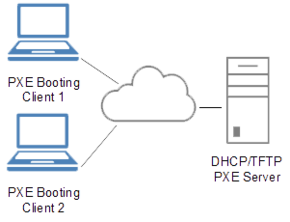
\includegraphics[width=0.5\textwidth]{290px-PXE_diagram.png}
%\includegraphics [width=3in] {file.eps} 
%将 file.eps 插入文档并且它的宽度被缩放到 3 英寸,高度也会 按相应的比例缩放。
%如果用 \textwidth 或 \em 等的函数来 指定宽度,而不是用像 3 英寸这样的固定尺寸,将会使你的 LATEX 文 档更具通用性。
%例如: \includegraphics [width=\textwidth] {graphics.eps} 
%将所插入图形缩放到和文本行的宽度一样宽。
%而下面的命令 
%\includegraphics [width=0.80\textwidth]{graphics.eps} 
%使得插入图形的宽度为文本行宽的 80%。
%当与 calc 宏包配合使用 时,下面的命令可令图形的宽度比文本行宽少 2 英寸: 
%\includegraphics [width=\textwidth-2.0in]{graphics.eps}
%---------------------
%原文:https://blog.csdn.net/sinat_36301420/article/details/79334728 
\end{figure}
\end{frame}


\begin{frame}
\frametitle{Network Prerequisites}
先来学习一些网络基础知识。
为了清晰,我们从网线中传输的1010开始,一步步构建到应用层。
\end{frame}




\begin{frame}
\frametitle{What's inside the twisted wire cable?}
双绞线中传输的1和0:
\begin{itemize}
\item 基本数据传输单位是\textbf{一个帧},在以太网规范 IEEE 802.3 中有详细描述,包括帧的格式(Premable,MAC,Payload,Checksum)和编码(4b/6b等)
\item 帧有广播帧(目标MAC为FF:FF:FF:FF:FF:FF)和普通帧(单播帧)的区别,请注意
\item 规定最大帧长度MTU,传统规范为1500;也要注意Jumbo Frame
\item 通过MAC地址识别接收和发送方;MAC地址理论上全球网卡唯一
\item 采用\textbf{载波监听与碰撞检测(CSMA/CD)}技术,允许通过共享媒介通信
\end{itemize}
\centering 问题:如何确定网络中计算机网卡的MAC地址?
\end{frame}

\begin{frame}
\frametitle{Network Topology, Hubs and Switches}
早期的互联网通过共享总线通信,所有计算机连接到同一根“网线”或同轴电缆上:
\begin{itemize}
\item 节约成本,不需要额外硬件
\item 但是,如果网线中任意一点故障,将导致整个网络不可用
\end{itemize}
\begin{figure}
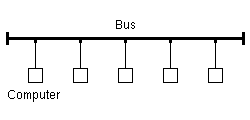
\includegraphics[width=0.5\textwidth]{Bustopologie.png}
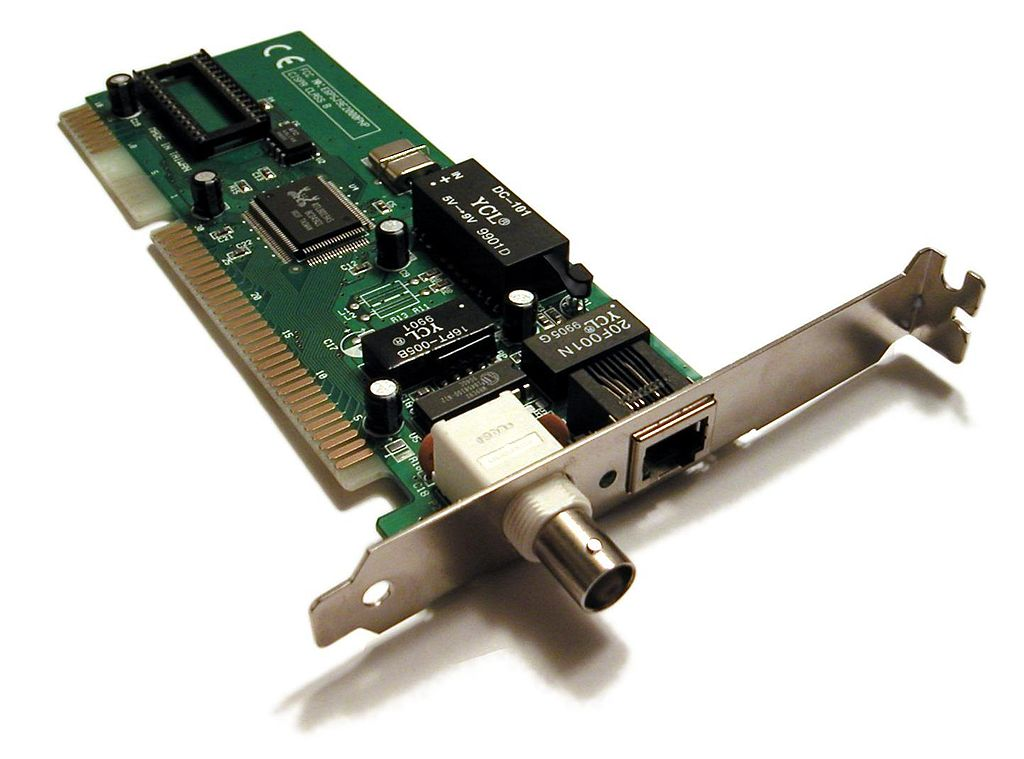
\includegraphics[width=0.4\textwidth]{1024px-Network_card.jpg}
\caption{总线型网络\ 与\ 一块同时支持同轴电缆和双绞线的ISA网卡}
\end{figure}
\end{frame}



\begin{frame}
\frametitle{Network Topology, Hubs and Switches}
为了提高容错,大家想到把拓扑结构改成星型,提高网络可靠性。中间的节点叫做 \textbf{集线器(Hub)}:
\begin{itemize}
\item 一个Hub基本可以理解为把几个端口的双绞线通过中继器放大信号后,直接连接在一起
\item 好处就是便宜!
\item 连接过远或过多Hub的情况下,CSMA/CD机制中的碰撞检测失效,导致帧不能正确传输;参见5-4-3规则等
\item 在高负载时,由于大量帧碰撞,系统吞吐量和延迟急剧恶化
\end{itemize}

\begin{figure}
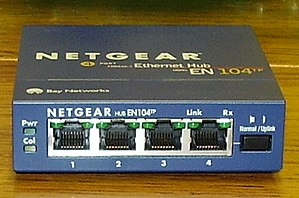
\includegraphics[width=0.3\textwidth]{300px-4_port_netgear_ethernet_hub.jpg}
\caption{四口以太网Hub,制造商NETGEAR}
\end{figure}
\end{frame}

\begin{frame}
\frametitle{Network Topology, Hubs and Switches}
为了解决高负载下帧碰撞降低网络性能的问题,人们想到了\textbf{交换机(Switch)}:
\begin{itemize}
\item 交换机使用了\textbf{存储-转发策略},隔离每个节点之间的普通帧。
\item 交换机内部维护一张端口和MAC地址的映射表,通过映射表转发包
\item 广播帧\footnote{为了方便,认为广播帧可达的计算机在同一个\textbf{广播域(Broadcast Domain)}中,单播帧可达的计算机在同一个\textbf{碰撞域(Collision Domain)}中}照例广播(除非用VLAN划分更小的子网),所以广播域与使用Hub相同
\end{itemize}
问题1:当交换机上电或连接新设备时,映射表如何建立?\\
问题2:可不可以仅仅使用交换机,构成互联网呢?
\end{frame}

\begin{frame}
\frametitle{Routers and the IP Protocol}
只使用交换机连广播域都没法隔离,并且只能单线连接\footnote{如果网络中有环,帧就会在环路中反复发送,直到耗尽交换机的全部交换能力。少院机房之前就搞过这个乌龙,还以为是交换机坏了}。对此,人们想到了\textbf{IP协议(Internet Protocol)}:
\begin{quote}
The Internet Protocol is designed for use in interconnected systems of packet-switched computer communication networks.  Such a system has been called a "catenet" [1].  The internet protocol provides for  transmitting blocks of data called datagrams from sources to destinations, where sources and destinations are hosts identified by fixed length addresses.  The internet protocol also provides for fragmentation and reassembly of long datagrams, if necessary, for transmission through "small packet" networks.
\end{quote}

节选自RFC 791,上面部分描述了IP协议的设计动机——为了包转发系统的互联,包的路由和不同系统允许最大帧长度不同的处理。
\end{frame}

\begin{frame}[fragile]
\frametitle{Routers and the IP Protocol}
\fontsize{9pt}{9pt}
\begin{verbatim}
 0                   1                   2                   3
 0 1 2 3 4 5 6 7 8 9 0 1 2 3 4 5 6 7 8 9 0 1 2 3 4 5 6 7 8 9 0 1
+-+-+-+-+-+-+-+-+-+-+-+-+-+-+-+-+-+-+-+-+-+-+-+-+-+-+-+-+-+-+-+-+
|Version|  IHL  |Type of Service|          Total Length         |
+-+-+-+-+-+-+-+-+-+-+-+-+-+-+-+-+-+-+-+-+-+-+-+-+-+-+-+-+-+-+-+-+
|         Identification        |Flags|      Fragment Offset    |
+-+-+-+-+-+-+-+-+-+-+-+-+-+-+-+-+-+-+-+-+-+-+-+-+-+-+-+-+-+-+-+-+
|  Time to Live |    Protocol   |         Header Checksum       |
+-+-+-+-+-+-+-+-+-+-+-+-+-+-+-+-+-+-+-+-+-+-+-+-+-+-+-+-+-+-+-+-+
|                       Source Address                          |
+-+-+-+-+-+-+-+-+-+-+-+-+-+-+-+-+-+-+-+-+-+-+-+-+-+-+-+-+-+-+-+-+
|                    Destination Address                        |
+-+-+-+-+-+-+-+-+-+-+-+-+-+-+-+-+-+-+-+-+-+-+-+-+-+-+-+-+-+-+-+-+
|                    Options                    |    Padding    |
+-+-+-+-+-+-+-+-+-+-+-+-+-+-+-+-+-+-+-+-+-+-+-+-+-+-+-+-+-+-+-+-+
\end{verbatim}
\fontsize{11pt}{11pt}
上面是一个IP包头,节选自RFC 791。
\end{frame}

\begin{frame}
\frametitle{Routers and the IP Protocol}
对于每一个在IP层工作的设备,都需要一个IP地址。
\begin{itemize}
\item 对于IPv4协议,地址长度为32位,采用点分二进制表示\\
例:\textbf{192.168.1.254} 对应的二进制地址
\item 定义一些特殊地址,用来实现特殊的功能
\begin{itemize}
\item 10.0.0.0/8 \footnote{此处/8表示子网掩码的前8位是1,即255.0.0.0。子网掩码一会介绍。} 172.16.0.0/12 192.168.0.0/16 用于私有地址
\item 127.0.0.0/8 用于回环地址
\item 其它请参见https://en.wikipedia.org/wiki/IPv4中的Special Use Addresses一节
\end{itemize}
\item 私有地址约定不能参与Internet上的路由\footnote{一会介绍。}。这表示,如果Internet上的路由器发现某个包的目的地址是私有地址,它就会被退回。
\end{itemize}
\end{frame}

\begin{frame}
\frametitle{Routers and the IP Protocol}
\textbf{路由(Routing)},即为每个IP数据包寻找道路。
\begin{enumerate}
\item mkdir ~/XcxSaikou
\item cp /etc/apt/source.list ~/XcxSaikou
\item cd ~/XcxSaikou
\item ls -l
\end{enumerate}
\end{frame}


\begin{frame}
\frametitle{What's under \textbf{/}?}
Mission 2: Find what's under "\textbf{/}"?
\end{frame}

\begin{frame}
\frametitle{What's under \textbf{/}?}
\begin{itemize}
\item \textbf{/home} - User home directories\\
In Unix, the directory \textbf{/home/your\_account} is the most decent place for you to store your personal data.
\item \textbf{/usr} - Executables, libraries, and shared resources that are not system critical
\item \textbf{/etc} - System-wide configuration files and system databases
\item \textbf{/dev} - Devices, such as hard disks, ttys and displays.
\item \textbf{/var} - Log files, print jobs, mails and temporaries
\item \textbf{/lib} - Shared libraries, kernel module or device drivers.
\item \textbf{/bin} - Binaries that should be available even when \textbf{/usr} haven't been mounted
\item $\cdots$
\end{itemize}
\end{frame}

\begin{frame}
\frametitle{Basic File Editing}
\begin{itemize}
\item User-friendly: \textbf{nano a.txt}
\item Experienced: \textbf{vim a.txt}
\item Obsolete: \textbf{ed a.txt}
\end{itemize}
Mission 3: Create a text file called "\textbf{Comments\_On\_Fruits.txt}" and write some words in it. You may use any of them if you like.
\end{frame}

\begin{frame}
\frametitle{Users and Permissions}
Users are entities who operate on this system.
\begin{itemize}
\item Every file and folder has an owner
\item Users can only Read/Write/eXecute when they have the permission
\item Use \textbf{ls -l} to see the permissions:\\
\end{itemize}
\begin{tabular}{llllll}
-rw-r--r-- & 1 & libreliu & sudo  &        38 Oct 15 23:29 & flag.txt\\
drwxr-xr-x &  5  & libreliu & sudo &       4096 Oct 18 20:37 & writeup\\
\end{tabular}


\end{frame}


\begin{frame}
\frametitle{SSH Operations}
SSH stands for \textit{Secure Shell}, a software suite and a protocol designed for delivering remote shell, file copying and port-forwarding.
\begin{itemize}
\item \textbf{ssh tempuser@192.168.4.233} - initiate a connection to remote machine, with username tempuser.\\
When username was not specified, the ssh client will attempts to connect with local username that's using.
\item \textbf{scp -r tempuser@192.168.4.233:/home/tempuser /home/tempuser/archive\_at\_remote} - copy files from remote machine by using \textit{Secure Copy} command
\end{itemize}

Mission 4: Try copying files \textbf{flag.txt} from my laptop by using the account I given.
\end{frame}



\end{document}